\section{Design Considerations and Open Challenges}

Before presenting the full protocol, we discuss several important design
considerations raised during protocol analysis. These address gaps not yet resolved
in the related literature and inform our protocol choices.

\subsection{Secure AST Issuance: Authenticating the Infrastructure}
\label{sec:ast_issuance}

A critical security requirement that existing anonymous credential schemes often
overlook is: \emph{how does the vehicle verify that it is communicating with a
legitimate AIS and not a rogue/fake infrastructure node?} Without this check, an
attacker could impersonate an AIS and issue malicious ASTs that pass the ZKP check
but contain incorrect validity windows or fabricated session identifiers, enabling
forged safety messages.

We address this with a \textbf{certificate-chain-authenticated AIS} design:

\begin{enumerate}
    \item The AIS is provisioned with a long-term certificate $\mathsf{cert}_{AIS}$
    issued and signed by the Trusted Authority:
    $\mathsf{cert}_{AIS} = (pk_{AIS},\ \mathsf{validity},\ \mathsf{Sign}_{sk_{TA}}(pk_{AIS} \| \mathsf{validity}))$.

    \item Before beginning AST acquisition, $V_i$ verifies the AIS certificate
    against $pk_{TA}$, which is pre-loaded into the OBU during vehicle registration.
    This is analogous to TLS server certificate verification.

    \item All AIS-issued ASTs carry a compact AIS-signed commitment:
    $\mathsf{sig}_{AIS} = \mathsf{Sign}_{sk_{AIS}}(H(\mathsf{AST}_i \| R_{current}))$,
    binding the token to the current Merkle root. This prevents an attacker from
    issuing a token pointing to a stale or fabricated root.

    \item Vehicles check $\mathsf{sig}_{AIS}$ before accepting any AST and before
    performing precomputation. If verification fails, the vehicle aborts the
    issuance session and may report the incident to the TA via a trusted out-of-band
    channel.
\end{enumerate}

This mechanism adds one ECDSA verification during AST acquisition---a one-time cost
per session that does not affect per-message online latency.

\subsection{AST Request Policy: When and How Often}
\label{sec:ast_policy}

A question left open by most anonymous credential schemes is: \emph{when exactly
should a vehicle request a new AST?} A naive fixed-interval policy is both
inefficient and privacy-leaking---fixed timing patterns are exploitable for traffic
analysis. We instead adopt an \textbf{event-driven request policy} governed by four
prioritised trigger conditions:

\begin{enumerate}
    \item \textbf{Proof cache below threshold $\theta_{cache}$.} When the number of
    remaining valid precomputed proof slots falls below $\theta_{cache} = 0.3$ (30\%)
    of total cache capacity, the vehicle must replenish before cache exhaustion
    mid-drive. This is the most operationally critical trigger.

    \item \textbf{AST approaching expiry.} When $t_{current} > t_{end} - T_{margin}$,
    where $T_{margin}$ is a renewal safety buffer set to 20\% of the total AST
    validity window, the vehicle must renew before expiry.

    \item \textbf{Epoch transition detected.} When the vehicle receives
    $R_{new} \neq R_{current}$ from an RSU or AIS, precomputed proof slots for the
    old root become stale after grace period $T_{grace}$. The vehicle requests a
    new AST and begins fresh precomputation immediately.

    \item \textbf{First infrastructure contact after offline period.} Upon
    re-establishing connectivity after any offline gap, the vehicle proactively
    checks conditions (1)--(3) and requests if needed.
\end{enumerate}

In addition, a vehicle applies an \textbf{opportunistic top-up} rule: if
infrastructure is available, the vehicle is stationary or in a low-mobility state,
and the proof cache is below full capacity, it requests a new AST to maximise the
cache for the next driving segment.

\paragraph{Privacy Implications of Request Timing.}
To mitigate timing fingerprinting from AST request patterns, the vehicle adds a
uniformly random delay $\delta \sim \mathcal{U}(0, \Delta_{jitter})$ before
initiating non-urgent requests (triggers~2 and opportunistic top-up). For urgent
triggers (1, 3, 4), no jitter is added to avoid cache depletion. We recommend
$\Delta_{jitter} = 30$\,s, preventing precise timing fingerprinting while remaining
small relative to the AST validity window.

\paragraph{Expected Request Frequency.}
For a representative AST validity window of 15--20 minutes and a proof cache sized
for $\approx$10 minutes of continuous BSM broadcasting at 10\,Hz (6000 proof slots),
the expected request frequency is approximately one request per 10--15 minutes---
comparable to the pseudonym rotation frequency in SCMS. Fig.~\ref{fig:ast_fsm}
summarises the complete event-driven policy as a finite state machine.

\begin{figure}[t]
    \centering
    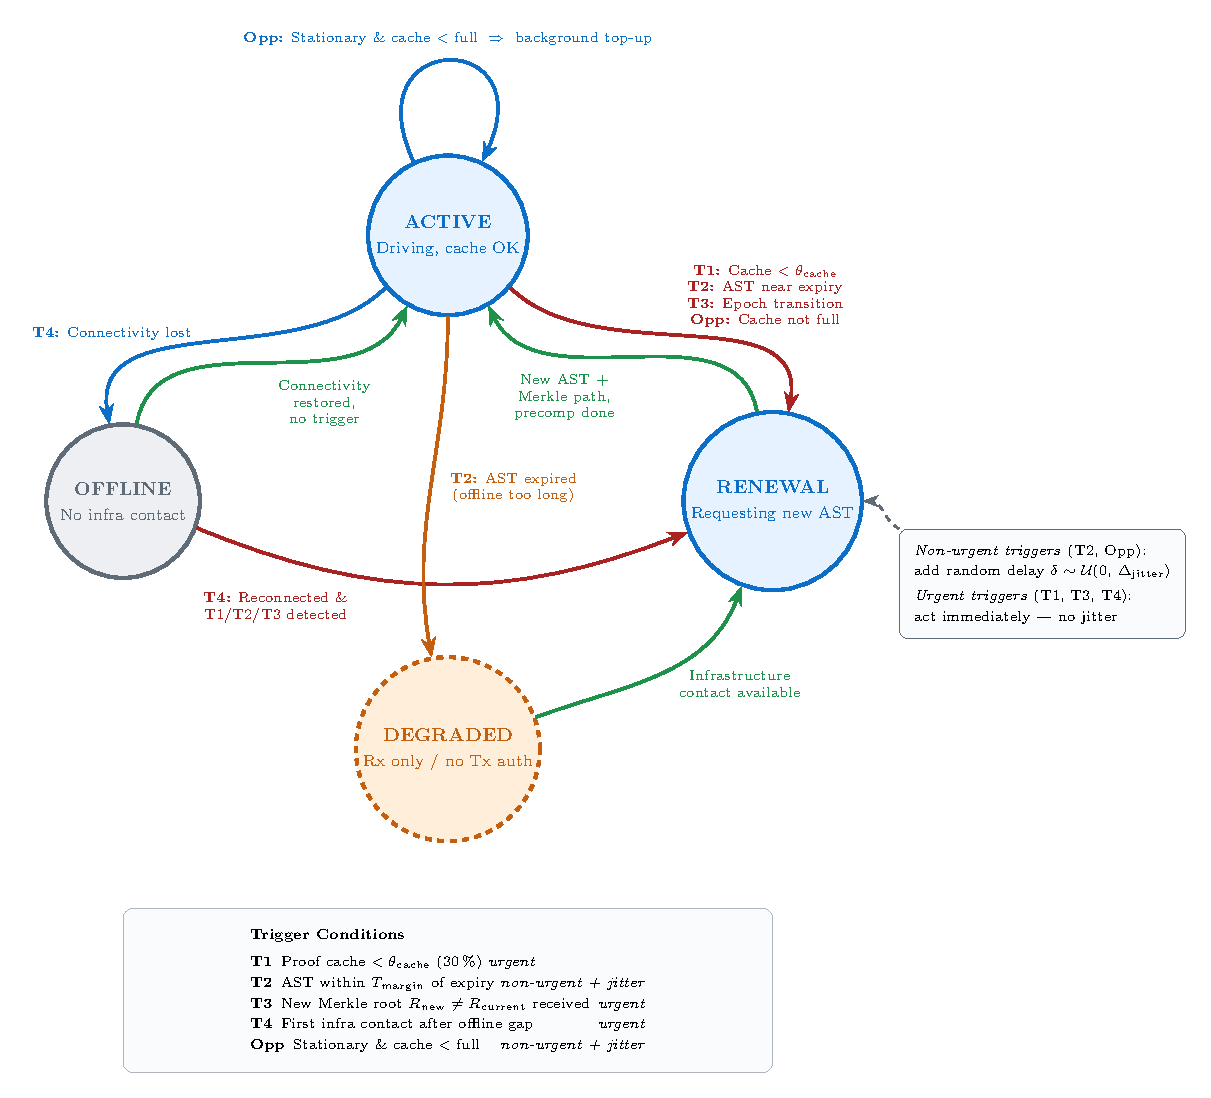
\includegraphics[width=\linewidth]{assets/ast-fsm.pdf}
    \caption{AST request policy finite state machine. States: \textsc{Active}
    (normal driving), \textsc{Offline} (no infrastructure contact), \textsc{Renewal}
    (requesting new AST), \textsc{Degraded} (AST expired, receive-only). Transitions
    are colour-coded: blue = normal flow, red = trigger-fired requests, green =
    recovery transitions, orange = degraded path. Non-urgent triggers (T2, Opp)
    add a random jitter delay $\delta \sim \mathcal{U}(0, \Delta_{\text{jitter}})$
    to prevent timing fingerprinting.}
    \label{fig:ast_fsm}
\end{figure}

\subsection{Epoch Management and Offline Resilience}
\label{sec:epoch}

The Merkle tree of active ASTs is maintained by the AIS and updated at epoch
boundaries. Each update changes the root $R$ and potentially invalidates AST
Merkle paths, creating a challenge for vehicles that are offline during an epoch
transition.

\paragraph{Epoch Duration and Overlap.}
Each AST spans at least two full epochs: $t_{end} - t_{start} \geq 2 \cdot T_{epoch}$.
A vehicle can therefore miss one complete epoch transition without its AST becoming
invalid.

\paragraph{Pre-fetched Merkle Paths for Future Epochs.}
During AST acquisition, the AIS provides the current Merkle path $\pi^{MT}_i$ and
pre-signed commitments for the next epoch root $R_{next}$ (if already computed),
allowing the vehicle to verify proofs against $R_{next}$ without re-contacting the
AIS. This approach is inspired by key chain commitment techniques used in broadcast
authentication protocols for vehicular networks~\cite{muhammad2024}.

\paragraph{Grace Period for Offline Vehicles.}
Verifier vehicles $V_V$ accept proofs referencing the \emph{previous} root $R_{prev}$
for a grace period $T_{grace}$ (e.g., 30 seconds) after each epoch transition.
After $T_{grace}$, only proofs referencing $R_{current}$ are accepted.

\paragraph{Root Dissemination.}
Updated Merkle roots are broadcast by RSUs as part of beacon messages. The root is
small (32 bytes for a Poseidon hash), so dissemination overhead is negligible.

\paragraph{Handling Vehicles Offline at AST Expiry.}
If a vehicle's AST expires while offline, it falls back to \emph{degraded mode}:
it continues to receive and verify messages from other vehicles but does not transmit
authenticated safety messages. The receive-only restriction is a \emph{cryptographic
necessity}: without a valid AST, the vehicle cannot construct a Groth16 proof
satisfying the three conditions of Phase~3, so any transmitted message would be
unconditionally rejected. This behaviour is consistent with IEEE~1609.2/SCMS, where
a vehicle with no valid credential is expected to cease broadcasting~\cite{ieee1609}.

\subsection{ZKP System Selection: Groth16 vs.\ PLONK vs.\ zk-STARK}
\label{sec:zkp_selection}

A natural question is why we select Groth16 rather than PLONK~\cite{gabizon2019plonk}
(which avoids a circuit-specific trusted setup) or zk-STARKs (which require no
trusted setup and offer post-quantum security). Table~\ref{tab:zkp_comparison}
provides a quantitative comparison; we argue that Groth16 is the uniquely
appropriate choice for V2V safety message authentication.

\begin{table}[t]
\centering
\caption{ZKP System Comparison for V2V Safety Message Authentication
(BN254, depth-16 circuit, $\sim$9{,}100 constraints)}
\label{tab:zkp_comparison}
\resizebox{\columnwidth}{!}{%
\begin{tabular}{@{}lccc@{}}
\toprule
\textbf{Property} & \textbf{Groth16} & \textbf{PLONK} & \textbf{zk-STARK} \\
\midrule
Proof size & $\approx$128\,B & $\approx$500--1000\,B & $\approx$50--200\,KB \\
Fits BSM packet ($<$1500\,B) & \checkmark\,(ample) & \checkmark\,(tight) & \texttimes\,(infeasible) \\
Verifier pairings & 3\,(constant) & $\sim$10 + poly evals & Poly-log \\
Prover time (rel.)~\cite{roelink2024,snark_stark_comparison2025} & 1$\times$ & $\sim$2.25--4$\times$ & $\sim$68$\times$ \\
Clean algebraic batch verify & \checkmark & Limited & \texttimes \\
Trusted setup & Circuit-specific & Universal SRS & None \\
Post-quantum & \texttimes & \texttimes & \checkmark \\
\bottomrule
\end{tabular}%
}
\end{table}

\subsubsection{Why Not PLONK?}

PLONK~\cite{gabizon2019plonk} offers a universal SRS and updatable trusted setup,
which are genuine advantages in environments where circuits evolve frequently. For
our application, these advantages do not materialize:

\textbf{Proof size} is the decisive constraint. A PLONK proof comprises 9
$\mathbb{G}_1$ elements plus 7 field elements, totalling 500--1000\,bytes depending
on encoding~\cite{roelink2024}. A Groth16 proof is exactly 128\,bytes. The BSM
payload itself (position, velocity, heading, brake status) occupies
$\approx$200--300\,bytes; a PLONK proof would consume $>$50\% of the remaining
1500-byte packet budget. Groth16's 128\,bytes uses only $\approx$9\% of the budget.

\textbf{Prover speed.} For circuits dominated by Poseidon-based Merkle hashing
(our case), PLONK is $\approx$2.25--4$\times$ slower than Groth16 due to higher
polynomial degree requirements for copy constraints~\cite{roelink2024}.

\textbf{Batch verification.} Groth16's three-point structure
$(A \in \mathbb{G}_1, B \in \mathbb{G}_2, C \in \mathbb{G}_1)$ admits clean
randomised linear combination, reducing $3k$ pairings to $k+3$ via multi-scalar
multiplication. PLONK batch verification requires aggregating multiple polynomial
commitment evaluations and does not achieve the same clean reduction~\cite{lipmaa2024polymath}.

\textbf{Universal SRS is irrelevant.} The V2V authentication circuit is fixed at
firmware deployment time---it encodes fixed operations (Merkle depth $d$, Poseidon
hashing, timestamp range check). A one-time ceremony per circuit version is
acceptable in the vehicular standards context, analogous to IEEE 1609.2's root CA
ceremony.

\subsubsection{Why Not zk-STARKs?}

zk-STARKs are post-quantum secure and require no trusted setup. However, their proof
sizes of 50--200\,KB and prover times $\approx$68$\times$ slower than Groth16 on
equivalent ARM hardware make them completely infeasible for 10\,Hz V2V
broadcasting~\cite{snark_stark_comparison2025}. A single STARK proof would exceed
the entire 802.11p packet size limit by a factor of 30--100.

\subsubsection{Post-Quantum Migration Path}

Groth16 on BN254 does not provide post-quantum security---a legitimate long-term
concern for systems with a 15--20 year deployment lifecycle. This is a known and
accepted tradeoff in current V2X standardization: IEEE 1609.2-2022 also relies on
ECDSA (P-256/P-384) with no post-quantum option. The anticipated migration path is
a firmware-level protocol version update in which the AIS performs a new trusted
setup ceremony for an updated circuit, analogous to CA root key rotation.
Post-quantum zk-SNARKs (lattice-based or hash-based constructions) represent a
natural future extension of this work.

\subsection{Groth16 Trusted Setup: Ceremony and Rationale}
\label{sec:trusted_setup}

Groth16 requires a two-phase structured reference string (SRS) generation:

\begin{itemize}
    \item \textbf{Phase 1 (Powers of Tau, Universal):} A multi-party computation
    (MPC) ceremony generating generic parameters $\{[\tau^i]_{G_1}, [\tau^i]_{G_2}\}$
    up to circuit depth $n$. This phase is circuit-independent. Existing publicly
    verifiable ceremonies (e.g., the Hermez/Polygon perpetual Powers of Tau
    ceremony supporting up to $2^{28}$ constraints) can be directly reused,
    eliminating the need to run Phase~1 from scratch~\cite{snarkjs_github}.

    \item \textbf{Phase 2 (Circuit-Specific):} A second MPC ceremony specialising
    the Phase~1 output to the ULP-V2V-Auth circuit. Participants include automotive
    OEMs, standardisation bodies (IEEE 1609 WG, ETSI ITS), and independent auditors.
    Security holds as long as at least one participant honestly deletes their
    contribution~\cite{bowe2017mpc}. The resulting $(\mathsf{pk}, \mathsf{vk})$ are
    embedded in OBU firmware during manufacturing, analogous to root CA certificates
    in devices today.
\end{itemize}

The trusted setup is a \textbf{one-time, offline} operation performed by the system
deployer. The proving key $\mathsf{pk}$ is pre-loaded into OBU RAM at startup
(avoiding I/O latency during operation). The verification key $\mathsf{vk}$ is
small (a few hundred bytes). Neither requires updating unless the circuit is
redesigned.

\subsection{Concurrent Sender/Receiver Operation}
\label{sec:concurrent}

In highway V2V, a vehicle is simultaneously a \emph{prover} (broadcasting its own
safety messages) and a \emph{verifier} (receiving and authenticating messages from
surrounding vehicles). We propose a \textbf{dual-module architecture}:

\paragraph{Sender Module (SM).}
\begin{itemize}
    \item \emph{Precomputation stage (background):} During AST acquisition and
    whenever CPU slack is available, the SM generates complete proof slots
    committed to predicted BSM content and caches them.
    \item \emph{Online stage (per-message):} At each broadcast interval, the SM
    retrieves the next precomputed slot, binds it to
    $h_m = H_{Poseidon}(m \| t_{current})$, completes the lightweight online proof
    step, and hands $(m, t_{current}, \pi, R)$ to the radio stack.
\end{itemize}

\paragraph{Receiver Module (RM).}
\begin{itemize}
    \item \emph{Collection window:} The RM buffers incoming
    $(m_j, t_j, \pi_j, R_j)$ tuples for a window $T_{window}$ (50--100\,ms).
    \item \emph{Batch verification:} At the end of each window, the RM performs
    batched Groth16 verification. Proofs referencing roots other than $R_{current}$
    (or $R_{prev}$ during $T_{grace}$) are immediately rejected.
    \item \emph{Priority filtering:} Inspired by EABA~\cite{zheng2018eaba}, the RM
    classifies messages by safety priority (e.g., emergency braking $>$ intersection
    warning $>$ routine BSM) and verifies high-priority messages individually and
    immediately, bypassing the batch window.
\end{itemize}

\paragraph{CPU Scheduling.}
The SM and RM run on separate threads (or cores on multi-core OBUs). Precomputation
has background priority; the online proof step and batch verification have real-time
priority. On a single-core OBU, precomputation is interleaved with idle periods
using a cooperative scheduling policy.

\subsection{Precomputation: Circuit-Level Analysis and Tolerability}
\label{sec:precomp_overhead}

Circuit-level analysis of our Circom implementation quantitatively validates the
offline/online decomposition. The constraint breakdown for the depth-16 circuit
($\sim$9{,}100 total) is:

\begin{itemize}
    \item Merkle path (16$\times$ Poseidon-2): $\approx$3{,}872 constraints (42.5\%)
    \item AST leaf hash (Poseidon-5): $\approx$580 constraints (6.4\%)
    \item Timestamp range checks (2$\times$ 32-bit LessEqThan): 64 constraints (0.7\%)
    \item Switcher and wiring: $\approx$4{,}342 constraints (47.7\%)
    \item \textbf{Message hash binding (Poseidon-2): $\approx$242 constraints (2.7\%)}
\end{itemize}

Exactly \textbf{97.3\% of constraints are message-independent}, motivating offline
precomputation of complete Groth16 proofs. The depth-16 circuit strengthens this
decomposition: the message-binding fraction \emph{decreases} from 4.3\% (depth-8)
to 2.7\% as the Merkle path dominates the larger circuit. In the proof-slot cache
model (Section~\ref{sec:bench_cache}), complete proofs are generated offline---each
committed to a predicted BSM content---and stored in a cache. The online step is
then reduced to (i)~dequeuing a pre-generated slot ($< 0.01$\,ms) and (ii)~computing
the Poseidon-2 hash $h_m = H_{\text{Poseidon}}(m \| t_{\text{current}})$ to verify
prediction accuracy ($\mathbf{0.439}$\,ms on RPi~4, directly measured over
5{,}000 runs). The total online cost of 0.439\,ms represents 0.44\% of the 100\,ms
BSM cycle---a $>$8{,}700$\times$ reduction from the full 3{,}841\,ms offline prove
time.

\paragraph{Proof cache sustainability.}
At 10\,Hz broadcasting, one proof slot is consumed per 100\,ms (600 slots/min).
On RPi~4, background precomputation with snarkjs ($\approx$3.84\,s/slot) produces
$\approx$15.6 slots/min, while the native C++ rapidsnark prover reduces this to
$\approx$1{,}422\,ms/slot ($\approx$42.2 slots/min), providing a $2.70\times$
improvement in cache fill rate. With dual-core scheduling, the production rate
($\approx$42/min with rapidsnark) is $14.2\times$ below the consumption rate of
600/min at 10\,Hz. Self-sustaining cache replenishment therefore requires
$14.2\times$ BN254 multi-scalar multiplication (MSM) acceleration over the
RPi~4 baseline---met at the NXP~S32G 25$\times$ acceleration tier or above
(quantified in Section~\ref{sec:experiment}).

For continuous highway operation without intermediate stops, two practical deployment
models address this gap. First, a \textbf{pre-departure fill}: a vehicle pre-generates
sufficient slots for the planned journey during stationary periods (overnight charging,
rest-stop dwell, toll-plaza queue). A 60-minute highway segment at 10\,Hz requires
36{,}000 slots ($\approx$7\,MB of OBU storage), generatable in $\approx$21 minutes
across four CPU cores at the NXP~S32G 10$\times$ tier---well within typical
pre-departure idle time. Second, for vehicles with NXP~S32G 25$\times$ tier or
dedicated ZKP accelerators, cache production exceeds consumption continuously,
requiring no pre-fill.

\paragraph{Hardware acceleration path.}
Automotive-grade processors (NXP S32G, Renesas R-Car H3) include hardware
accelerators for elliptic curve point operations. An important distinction applies:
standard HSE acceleration targets single-point ECDSA operations, while Groth16
proving requires \emph{multi-scalar multiplication} (MSM)---a qualitatively
different workload. At the NXP~S32G 25$\times$ MSM tier, offline prove time drops
to $\approx$57\,ms/slot (self-sustaining); at the 10$\times$ tier ($\approx$142\,ms),
pre-departure fill covers highway trips as described above. Online binding remains
$<$2\,ms regardless of prove speed.

\paragraph{Storage overhead.}
Each precomputed proof slot requires $\approx$2--3 group elements plus the Merkle
path evaluation. For $n=2^{16}$ active ASTs, this is $16 \times 32 = 512$ bytes
per slot; maintaining 16 slots requires $\approx$5--8\,KB of secure storage---well
within OBU capabilities.

\paragraph{Design variant: one-time key binding.}
The position pre-commitment constraint is an artifact of embedding message binding
inside the ZKP circuit via $h_m = H_{\mathit{Poseidon}}(m \| t)$. An alternative
design commits a per-slot \emph{one-time keypair} $(sk^{(s)}_{\mathit{ot}},
pk^{(s)}_{\mathit{ot}})$ inside the proof instead of message content. At broadcast
time, the vehicle signs the actual BSM with $sk^{(s)}_{\mathit{ot}}$ (0.199\,ms
ECDSA-P256 sign), and the receiver verifies both the ZKP proof and the one-time
signature. This eliminates position prediction entirely: proofs are content-agnostic
at generation time and can be used for any BSM---including unpredicted emergency
events---without slot discarding. The tradeoff is $\approx$96 additional bytes per
packet (64\,B one-time signature $+$ 32\,B $pk_{\mathit{ot}}$ in public inputs) and
the need to generate a fresh keypair per slot. We adopt the current Poseidon-binding
design for its smaller packet footprint and simpler circuit; the one-time key variant
is a natural extension for deployments where prediction accuracy is a concern.
